\chapter{Introduction}
\label{cap:introduction}
In 1952 in the laboratories of the University of Cambridge as an example of a doctoral thesis was created "OXO", the transposition of "Tic-tac-toe" as a computer game. This is usually considered technically the first video game. In 1958 a physics professor at Brookhaven National Laboratory created the game "Tennis for Two", which had the task of simulating the physical laws that could be found in a tennis match: the istrument used was an oscilloscope.

In 1961, six young scientists from Massachusetts Institute of Technology programmed, on a PDP-1\footnote{Programmed Data Processor-1 a computer from Digital Equipment Corporation.} computer, the first properly designed video game: "Spacewar!".

Two months later two electrical engineers N. Bushnell and T. Dabney finished their version of "Spacewar!" produced on a large scale (1,500 copies), but the game was not, however, a great success due to the high difficulty. Bushnell, after the not particularly successful experiment, however, decided to insist with video games, but producing them on his own: thus Atari was born. Atari's first arcade game was the industry's first big hit: "Pong", released in late 1972, which roughly reproduces the mechanics of ping pong. Atari sold 19,000 "Pong" cabinets and soon many imitators followed suit. At the end of the decade the golden age of arcade video games began.

For fifteen years now, the economic importance of video games in public places has considerably decreased\footnote{Except in Japan.} in favor of video games for personal computers, consoles and more recently for mobile devices. For this reason, the term arcade video game is often used to refer to the generation of "classic" arcades\cite{High_Score}.

\section{Cloud gaming}
Cloud gaming, is a type of online service that operate in a similar way to remote desktop and video on demand. Video games are stored and run remotely on a provider's dedicated hardware, they are streamed as a movie to a player's device via client. The client manages the player's inputs, which are sent to the server and executed in the game.

This type of approach offers many advantages, including making the game more easily accessible without having to download and install it locally, it is compatible with computers and smart phones, even on smart tv when used with a wifi gamepad. Several services may offer some additional functions to make the most of this model, a spectator can join a player's session and temporarily take control of the game, if authorized by the player himself.

It also definitively solves a problem that has existed since the days of compact cassettes and floppy disks: piracy.

The rapid development of the broadband networks and the continuously falling subscription costs made this method, today, a reality.

\section{Existing cloud gaming services}
The first hints of cloud gaming for the general public only came around 2010. One of the first platforms created to allow gamers from all over the world to experience the thrill of streaming gaming was "OnLive" by OL2. Presented at GDC\footnote{GDC: Game Developers Conference, an annual conference for video game developers.} 2009, then launched on the market in June 2010. Players could purchase games on the platform or play games from their Steam\footnote{Steam is a video game digital distribution service by Valve.} library\footnote{Video game digital library is the collections of video games purchased by an user.}.

In 2012, Gaikai inaugurated its cloud gaming service, the company mainly focused on using cloud gaming as a form of online advertising for video games, where users would have the opportunity to access video game demos.

OnLive and Gaikai were acquired by Sony and their resources were used as the basis for a cloud gaming service known as "Playstation Now".

In 2013, Nvidia introduced "GeForce Now", a cloud gaming service integrated in their "Shield TV\footnote{Nvidia Shield TV is an Android TV-based digital media player produced by Nvidia.}" device. In 2017, the company began expanding its service to PC, including support for importing a user's Steam library.

In May 2018, Electronic Arts acquired some cloud gaming assets from GameFly. EA\footnote{EA: Electronic Arts.} later announced "Project Atlas", a project that explored the integration of artificial intelligence and machine learning, making the platform dynamic, social and cross platform.

Microsoft at E3\footnote{E3: Electronic Entertainment Expo, a trade event for the video game industry.} 2018 teased his "Xbox Cloud Gaming" service.

At GDC 2019, Google officially announced its "Stadia" cloud gaming service, out for November 19 of the same year.

On September 24, 2020, a new service called "Luna" was announced by Amazon\cite{Cloud_gaming_history}.

But let's see the current cloud gaming landscape.

\subsection{Utomik}
The Utomik platform launched commercially in 2008 and has been in service since. Games to be played in a browser need the proprietary Utomik Player plugin. The platform offer an SDK\footnote{SDK: Software development kit, a collection of software development tools.}, plugin and online service to create, launch, maintain and monitor games\cite{Utomik}.

\subsection{Microsoft - Xbox Cloud Gaming}
Microsoft teased the service at E3 2018. The service is available for subscribers of Xbox Game Pass Ultimate from September 15, 2020. The platform offer the existing library of Xbox games and add new games from the Xbox Series X. The service is designed to work with phones (currently only Android), either with touchscreen controls or Xbox controller over Bluetooth.\cite{Xbox_Game_Pass_cloud_gaming}.

\subsection{Project Atlas}
In May 2018 Electronic Arts has unveiled its cloud-native gaming platform called Project Atlas, which aims to make numerous playable titles available through the company's servers and to provide a gaming experience never tried before thanks to the support of artificial intelligence. The platform intends to offer a cloud gaming experience that consists of truly living universes, which change with the passage of time, with interaction with other players and under the influence of the outside world. In these processes, the support of artificial intelligence and the learning of the habits and preferences of the players would play a fundamental role. It also offers a dynamic game client, which allows users to stream a title while they wait for the download to complete on their device's storage disk.\cite{Project_Atlas}.

\subsection{Nvidia - GeForce Now}
GeForce Now is Nvidia's cloud gaming service launched in beta in January 2017, and officially in February 2020. GeForce Now allows users to remotely access (via streaming) a virtual computer, where they can install games purchased on Steam, Ubisoft Connect\footnote{Ubisoft Connect is a digital distribution, digital rights management, multiplayer and communications service developed by Ubisoft.} or Epic Games Store\footnote{Epic Games Store is a digital video game storefront operated by Epic Games.}. The service can be used on Windows, macOS, iOS, Android or Nvidia Shield TV.\cite{GeForce_Now}.

\subsection{Sony - PlayStation Now}
PlayStation Now is a cloud gaming subscription service based on Gaikai's cloud technology and Microsoft Azure. Was presented during CES\footnote{CES: Consumer Electronics Show, an annual event that hosts presentations of new products and technologies in the consumer electronics industry.} 2014. It has been available since January 2015 in North America, in September in Japan and UK. The service started operating in Europe gradually from August 2017 to March 2019. The services allows the user to play PlayStation titles (from the games catalog of PS2, PS3 and PS4) on PS4, PS5 and Windows.\cite{PlayStation_Now}.

\subsection{Google - Stadia}
Stadia is a cloud gaming platform released in November 2019, but is only available in Europe and United States. On the platform the user can buy games or subscribe to the service in order to access to the games catalog.

Google has created the Stadia controller that connects via wifi directly to the service and make possible to play on a TV (installing the app or using a Chromecast\footnote{Google Chromecast is digital media players for internet-streamed audio-visual content}). You can play with mouse and keyboard or controller using the Chrome browser on any PC. There is a mobile app that supports touch screen controls and bluetooth gamepads.

The platoform offer some interesting feauture like: share the gameplay via a live stream on YouTube; Crowd Play which allows viewers to join the multiplayer games they are watching; Stream Connect that allow the user to share the game screen to other players in the same game; State Share that allow players to share their save state\cite{Google_Stadia}.

\subsection{Amazon - Luna}
Luna was announced on September 24, 2020, with ‘early access’ available to subscribers by invitation beginning on October 20, 2020. Amazon Luna will have 100 different games at launch and will be powered by AWS. Luna will have integration with Twitch. Amazon has partnered with Ubisoft to create a gaming channel (with an additional costs) exclusive to Luna, which will give Luna subscribers access to Ubisoft's titles the same day they release\cite{Amazon_Luna}.


\section{Proposed system}
A key feature of the system is usability and for this reason, on the client side, the web browser was the most obvious choice.
There are some streaming technology in HTML5: HLS, DASH, Websocket and WebRTC.

HLS is the most popular high-latency streaming protocol over HTTP for VOD (pre-recorded video).

DASH is an adaptive bitrate streaming technique that enables high quality streaming of media content over HTTP.

Websocket it is TCP based, but with lower latency than HLS and DASH.

WebRTC is based on SRTP, therefore to get RTP stream on the browser a WebRTC server is needed.

Since this project is designed for retrograming stands and to be performed on a local network within trade fairs and IT events, the transmission takes place on a WiFi LAN network, so the difference in speed between TCP and UDP becomes negligible, therefore the choice fell on WebSocket because it is a communication protocol standardized by 2011, it is fully supported by all the modern browsers, it is simple and does not require the use of additional protocols or complex configuration\cite{Audio_and_video_delivery}.


\begin{figure}[H]
	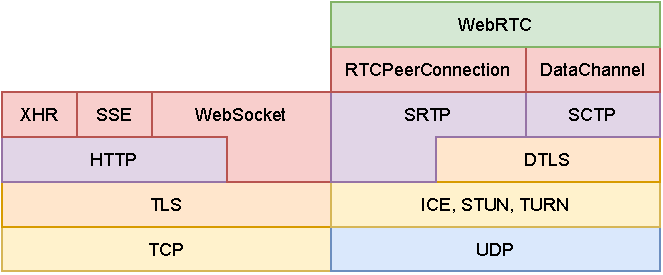
\includegraphics[width=\linewidth]{immagini/webprotocols}
	\caption{High-level browser networking APIs, protocols, and services }
	\label{fig:webprotocols}
\end{figure}

Lorem ipsum dolor sit amet, consectetur adipiscing elit, sed do eiusmod tempor incididunt ut labore et dolore magna aliqua. Ut enim ad minim veniam, quis nostrud exercitation ullamco laboris nisi ut aliquip ex ea commodo consequat. Duis aute irure dolor in reprehenderit in voluptate velit esse cillum dolore eu fugiat nulla pariatur. Excepteur sint occaecat cupidatat non proident, sunt in culpa qui officia deserunt mollit anim id est laborum.

\begin{figure}[H]
	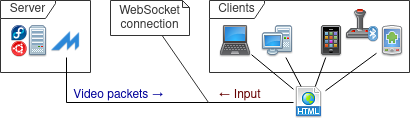
\includegraphics[width=\linewidth]{immagini/proposed_system}
	\caption{System overview}
	\label{fig:proposed_system}
\end{figure}


Lorem ipsum dolor sit amet, consectetur adipiscing elit, sed do eiusmod tempor incididunt ut labore et dolore magna aliqua. Ut enim ad minim veniam, quis nostrud exercitation ullamco laboris nisi ut aliquip ex ea commodo consequat. Duis aute irure dolor in reprehenderit in voluptate velit esse cillum dolore eu fugiat nulla pariatur. Excepteur sint occaecat cupidatat non proident, sunt in culpa qui officia deserunt mollit anim id est laborum\cite{High_Performance_Browser_Networking}.

Lorem ipsum dolor sit amet, consectetur adipiscing elit, sed do eiusmod tempor incididunt ut labore et dolore magna aliqua. Ut enim ad minim veniam, quis nostrud exercitation ullamco laboris nisi ut aliquip ex ea commodo consequat. Duis aute irure dolor in reprehenderit in voluptate velit esse cillum dolore eu fugiat nulla pariatur. Excepteur sint occaecat cupidatat non proident, sunt in culpa qui officia deserunt mollit anim id est laborum.